\section{线段点共享优化技术}
\label{sec6:LixelsAggregaion}

范围森林法和动态范围森林法在单个线段点上的查询表现出高效的性能,然而不同线段点之间的查询任然是独立的,这是基于核密度估计法的另一个瓶颈。在本章中,我们将介绍一种专门用于多项式核函数的优化方法,称为线段点共享优化。

原始算法中的海量计算来源于不同的线段点会在索引上产生不同的查询。特别地,如果查询的区间范围足够大,如图~\ref{fig:LS_1}所示,该聚合集将会包含该边上的所有数据点。此时这些数据点对其他线段点的贡献具有相似性。

\begin{figure}[h]\centering
    \scalebox{0.8}[0.8]{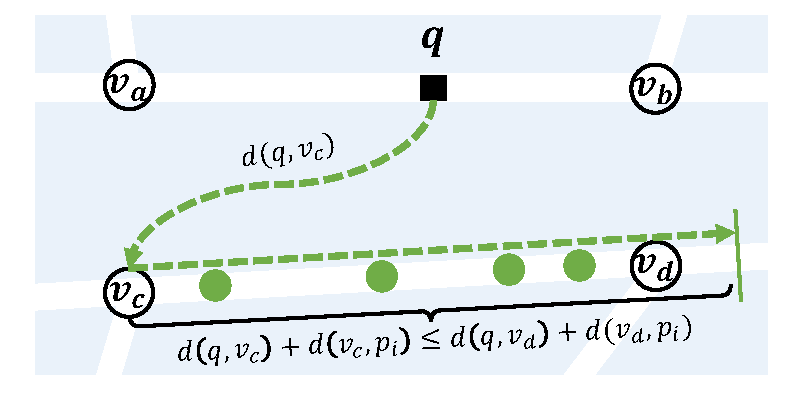
\includegraphics{./figures/LS_1.pdf}}
    \caption{一个支配边的例子。从 $q$ 到所有数据点的最短路径都会经过 $v_c$。}
    \label{fig:LS_1}
\end{figure}

\subsection{支配情况的判定}

具体来说,如果边$(v_a, v_b)$上的所有线段点都满足该条件,即查询的区间范围能够覆盖整条边$(v_c, v_d)$,我们称之为“支配”。例如在图~\ref{fig:LS_1}中,边 $(v_c, v_d)$ 在 $v_c$ 方向上被支配,因为从所有线段点 $q_i$ 到所有数据点的最短路径都会经过 $v_c$。形式化地说,对于所有线段点$q_i \in (v_a, v_b)$和数据点$p_i \in (v_c, v_d)$,支配情况有以下两个条件:
\begin{equation*}
% \label{eq:LS_1}
\begin{aligned}
    d(q_i, v_c) + d(v_c, p_i) &\le b_s \\
    d(q_i, v_c) + d(v_c, p_i) &\le d(q_i, v_d) + d(v_d, p_i) \\
\end{aligned}
\end{equation*}
第一个条件表示所有的数据点都在空间带宽范围内。考虑最坏的情况,$d(v_c, p_i)$为整条边$d(v_c, v_d)$的长度,$d(q_i, v_c)$为环$v_c {\rightarrow} v_a {\rightarrow} v_b {\rightarrow} v_c$的长度的一半,即$C / 2$,其中 $C = d(v_c, v_a) + d(v_a, v_b) + d(v_b, v_c)$ 是环的长度。

第二个条件表示所有的数据点都必须离 $v_c$ 更近,可以被改写为:
\begin{equation*}
    \max_{q_i}\{d(q_i, v_c) - d(q_i, v_d)\} \le \min_{p_i}\{d(v_d, p_i) - d(v_c, p_i)\}
\end{equation*} 
其中不等号右边最小值函数内的表达式具有单调性,因此$p_{n_e}$取到最小值;然而,不等号左边部分无法直接得到。事实上,有如下引理:
\begin{lemma}
    \label{lemma:LS_1}
    $d(q_i, v_c) - d(q_i, v_d)$的最大值最多只会在4个固定的地方出现,即只需要对4个$q_i$计算。
\end{lemma}
\begin{figure}[h]\centering
    \scalebox{0.8}[0.8]{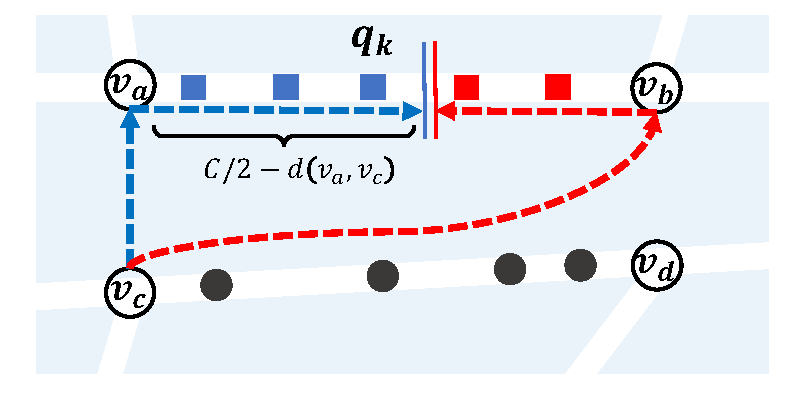
\includegraphics{./figures/LS_2.pdf}}
    \caption{一个支配边的例子。从 $v_c$ 出发到所有线段点的最短路径有两种路线,分别经过$v_a$ 或 $v_b$。}
    \label{fig:LS_2}
\end{figure}
\begin{proof}
    如图~\ref{fig:LS_2}所示,$d(q_i, v_c)$的最短路径一定是左边一部分从 $v_a$经过(用蓝色表示)而右边一部分从$v_b$经过(用红色表示)。因此,$d(q_i, v_c)$的值一定在 $q_1 \sim q_k$ 单调递增,而在$q_{k+1} \sim q_{l_e}$ 单调递减,其中 $k$ 如图所示两段的分割点,$l_e$ 表示边$(v_a, v_b)$上的线段点数量,且两段的公差分别为 $g$ 和 $-g$。

    $v_d$ 一侧的情况同理。$d(q_i, v_d)$的值一定在$q_1 \sim q_{k'}$单调递增,而在$q_{{k'}+1} \sim q_{l_e}$ 单调递减,其中 $k'$ 是另一个分割点,且两段的公差同样分别为 $g$ 和 $-g$。

    此时$d(q_i, v_c) - d(q_i, v_d)$就变成两个双等差数列的差,$q_1 \sim q_{\min\{k,k'\}}$部分和$q_{\max\{k,k'\}+1} \sim q_{l_e}$,两个数列的单调性相同,所以差值为定值。$q_{\min\{k,k'\}+1} \sim q_{\max\{k,k'\}}$部分,两个数列的单调性相反,此时结果仍然是一个等差数列,且公差为 $2g$或$-2g$。

    综上所述,只需要检验四个位置即可确定最大值,即 $k$,$k+1$,$k'$ 和 $k'+1$。
\end{proof}

\subsection{支配情况的计算}

利用引理~\ref{lemma:LS_1}我们可以快速地判断一条边存在支配情况。如果一条边被支配,那么公式(\ref{eq:aggregate})中的聚合向量 $\mathbf{A}$ 对所有线段点都是相同的。此时,整个核密度公式中唯一的变量就是$d(q, v_c)$,且最高次数为一,即:
\begin{equation*}
    F_e(q_i) = \alpha \cdot d(q_i, v_c) + \beta
\end{equation*}
并且,相邻两个线段点的核密度值之差为:
\begin{equation*}
    F_e(q_i) - F_e(q_{i-1}) = \alpha \cdot (d(q_i, v_c) - d(q_{i-1}, v_c)) = \alpha \cdot \Delta(q_i)
\end{equation*}


引理\ref{lemma:LS_1}已经说明了 $d(q_i, v_c)$ 由两个单调数列组成,且分割点为 $k$。因此,核密度值的一阶差分$\Delta(q_i)$为定值(除了分割点 $k$),二阶差分$\Delta^2(q_i)$则为零(除了分割点$k$)。图~\ref{fig:LS_3}展示了核密度值及它们的一阶二阶差分,我们只需要在二阶差分上更新两个值,就可以记录所有线段点的核密度值。

\begin{figure}[h!]\centering
    \scalebox{0.6}[0.6]{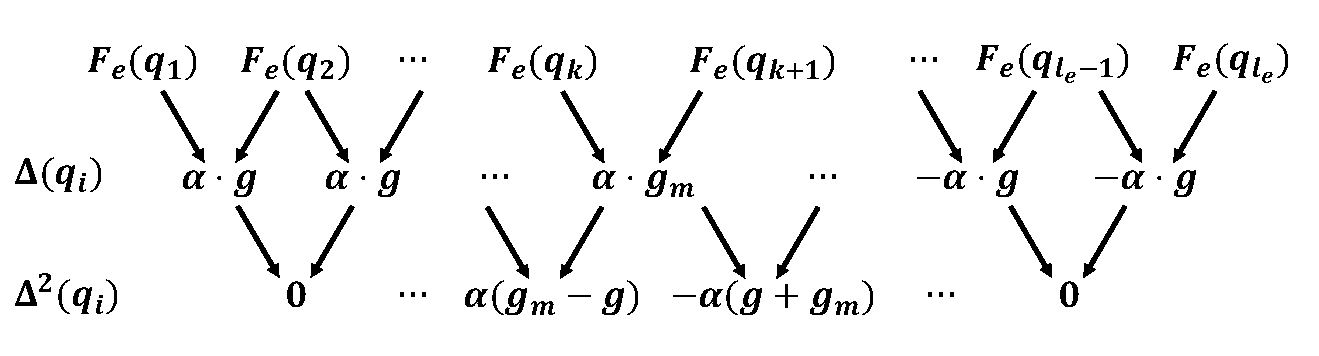
\includegraphics{./figures/LS_3.pdf}}
    \caption{线段点的核密度的一阶差分$\Delta(q_i)$和二阶差分$\Delta^2(q_i)$的可视化表示。二阶差分$\Delta^2(q_i)$除了分界点 $k$ 附近的两个值,其他全为零。}
    \label{fig:LS_3}
\end{figure}

注意到两个数组求和后的差分数组等价于分别差分后再相加,对于其他被支配的边,我们同样只需要再二阶差分上更新,最后依次还原成一阶差分和原数组即可。

最后,我们说明如何定位分割点 $k$。如图~\ref{fig:LS_2}所示,$q_k$ 是选择通过 $v_a$ 的最远的线段点,因此:
\begin{equation*}
    k = \left\lceil \frac{C/2 - d(v_a, v_c)}{g} + 0.5 \right\rceil
\end{equation*}
这里额外增加的 $0.5$ 是因为我们使用线段点的中点作为距离度量点,需要保证 $q_k$ 所对应的中点必须在这个范围内。

最后,一旦得到了 $k$,我们就能得到需要更新的值:
\begin{equation*}
    g_m = d(q_{k+1}, v_c) - d(q_k, v_c)
\end{equation*}


\subsection{越界情况的判定}

图~\ref{fig:LS_1}展示了如果聚合集包含了所有的数据点,可以进行一些优化。另一方面,如果聚合集不包含任意数据点,我们同样可以跳过这一过程。具体来说,我们有如下判定条件:
\begin{equation*}
\begin{aligned}
    d(q_i, v_c) + d(v_c, p_i) > b_s \\
    d(q_i, v_d) + d(v_d, p_i) > b_s
\end{aligned}
\end{equation*}
即所有的数据点都超出了空间范围带宽。考虑最坏的情况,$d(v_c, p_i) = d(v_d, p_i) = 0$,此时$d(q_i, v_c)$ 和 $d(q_i, v_d)$的最小值只会在两个端点$q_1$ 或 $q_{l_e}$出现。如果这两个线段点都距离很远了,那么整条边都可以被跳过。


\subsection{带线段点共享优化的框架}

算法~\ref{algo:LixelSharing}是经过线段点共享优化后的框架。首先,第3-5行会分别寻找支配边集合$E_d$,越界边集合 $E_o$,以及其他边 $E_q$。对于支配边,只需要更新核密度的二阶差分并恢复即可。接着使用原始流程计算其他边的核密度。

\begin{algorithm}[h]
	\caption{Lixel Sharing Framework}
	\label{algo:LixelSharing}
	\DontPrintSemicolon
	\SetKwComment{comment}{$\triangleright$ }{}
	
    \For{each edge $(v_a, v_b)$}{
        Get shared shortest path distance \\
        $E_d \leftarrow$ dominated edges \\
        $E_o \leftarrow$ out-of-bandwidth edges \\
        $E_q \leftarrow E \backslash (E_d \cup E_o$) \\
        \For{each edge $e \in E_d$}{
            update $\Delta^2(q_i)$
        }
        recover $F(q_i)$ from $\Delta(q_i)$ and $\Delta^2(q_i)$
        
        \For{each lixel $q_i \in (v_a, v_b)$}{
            \For{each edge $e \in E_q$}{
                compute $F_e(q_i)$ \\
                $F(q_i) \leftarrow F(q_i) + F_e(q_i)$
            }
	    }
    }
\end{algorithm}

\begin{lemma}
    算法~\ref{algo:LixelSharing}的时间复杂度为$O(\vert E \vert \cdot T_{sp} + \vert E \vert^2 + L \cdot \vert E_q \vert \cdot \log \frac{N}{E_q})$。
\end{lemma}
\begin{proof}
    第2行计算最短路径花费 $O(\vert E \vert \cdot T_{sp})$;第3-5行判定支配边花费$O(\vert E \vert)$;第6-7行计算支配边的核密度花费$O(\vert E_d \vert)$;第8行恢复操作在所有边上总共花费$O(L)$;第8-12行调用传统RFS算法会花费$O(L \cdot (\vert E_q \vert \log \frac{N}{\vert E_q \vert}))$。因此总时间复杂度为$O(\vert E \vert \cdot T_{sp} + \vert E \vert^2 + L \cdot \vert E_q \vert \cdot \log \frac{N}{E_q})$。
\end{proof}

算法~\ref{algo:LixelSharing}的效率提升主要由实际需要查询的边集$E_q$的大小所决定。在最坏情况下,没有边被支配或越界,此时$E_q = E$,即没有任何提升。如果$E_q$较小,则复杂度会有显著的减少。
